\documentclass[10pt,a4paper]{article}
\usepackage{amsmath}
\usepackage[
    colorlinks,
    citecolor=blue!70!black,
    linkcolor=blue!70!black,
    urlcolor=blue!70!black
]{hyperref}
\usepackage{tikz}
\usetikzlibrary{patterns}
\usepackage{xcolor}

\begin{document}

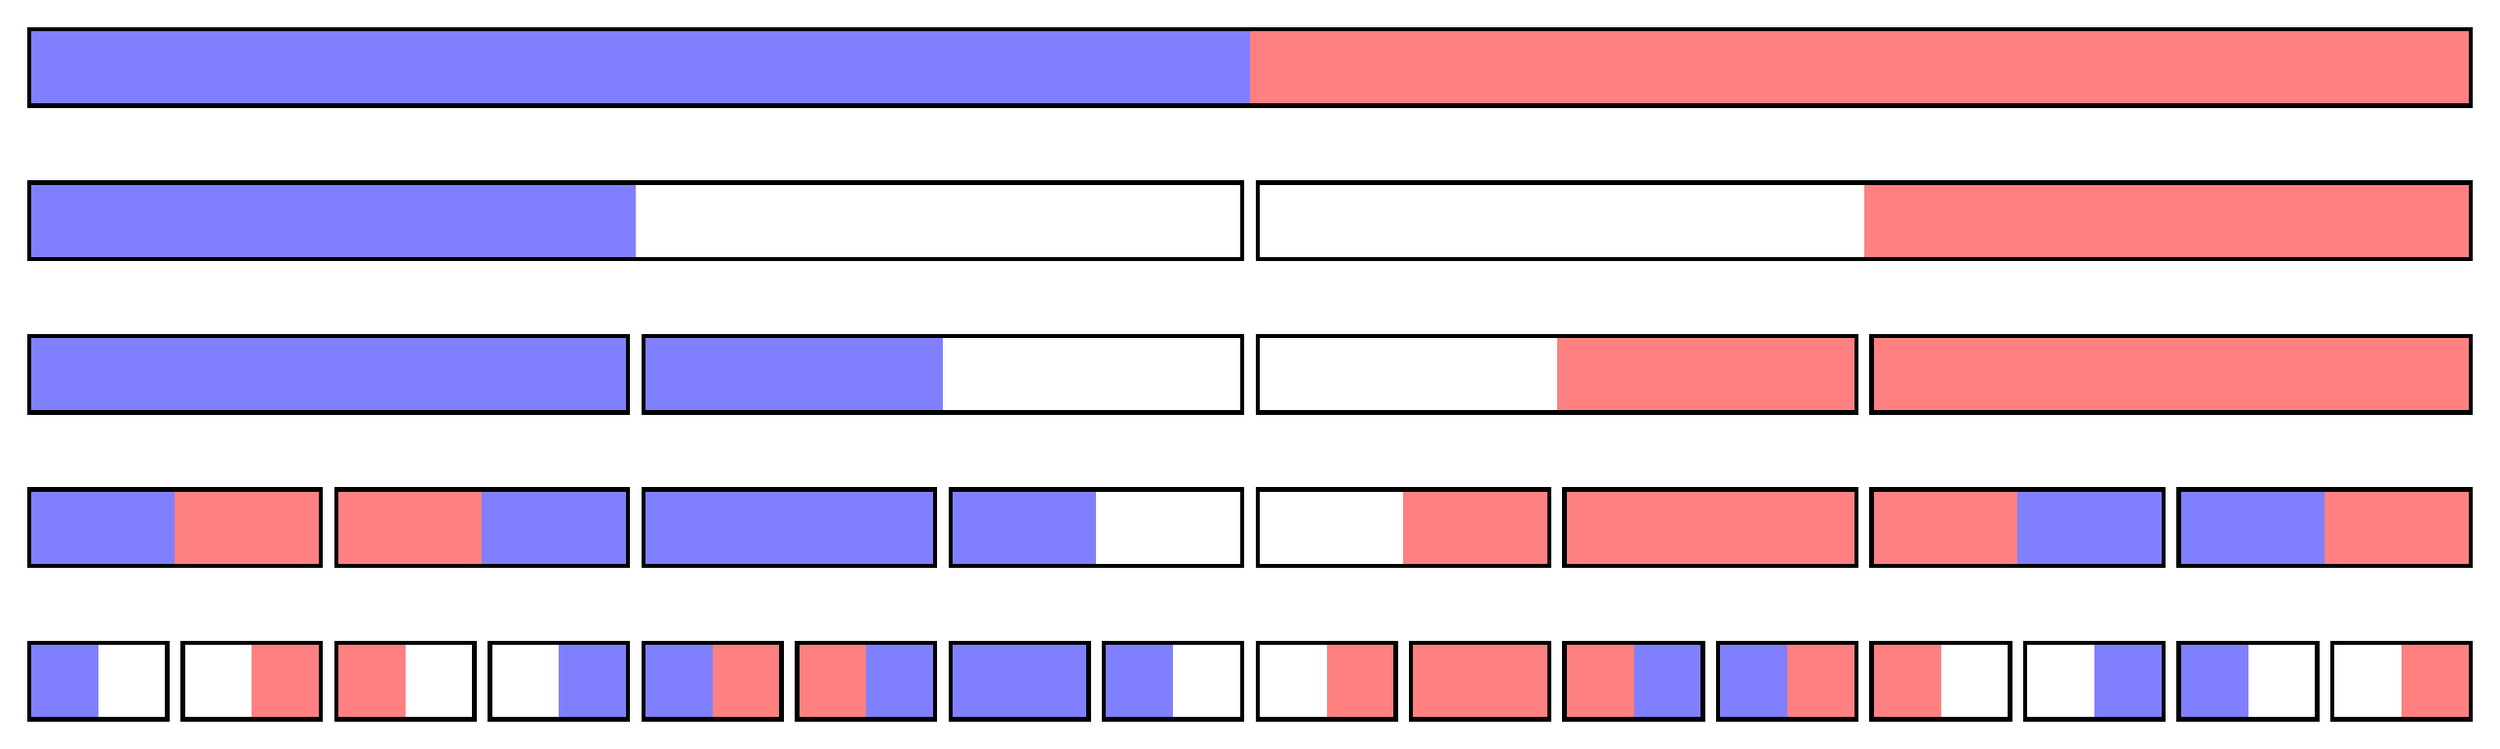
\begin{tikzpicture}
                \fill[blue!50] (0+.1,8) rectangle (16,9);
        \fill[red!50] (16,8) rectangle (32-.1,9);
        \draw[ultra thick] (0+.1,8) rectangle (32-.1,9);
        \fill[blue!50] (0+.1,6) rectangle (8,7);
        \fill[red!50] (24,6) rectangle (32-.1,7);
        \draw[ultra thick] (0+.1,6) rectangle (16-.1,7);
        \draw[ultra thick] (16+.1,6) rectangle (32-.1,7);
        \fill[blue!50] (0+.1,4) rectangle (4,5);
        \fill[blue!50] (4,4) rectangle (8-.1,5);
        \fill[blue!50] (8+.1,4) rectangle (12,5);
        \fill[red!50] (20,4) rectangle (24-.1,5);
        \fill[red!50] (24+.1,4) rectangle (28,5);
        \fill[red!50] (28,4) rectangle (32-.1,5);
        \draw[ultra thick] (0+.1,4) rectangle (8-.1,5);
        \draw[ultra thick] (8+.1,4) rectangle (16-.1,5);
        \draw[ultra thick] (16+.1,4) rectangle (24-.1,5);
        \draw[ultra thick] (24+.1,4) rectangle (32-.1,5);
        \fill[blue!50] (0+.1,2) rectangle (2,3);
        \fill[red!50] (2,2) rectangle (4-.1,3);
        \fill[red!50] (4+.1,2) rectangle (6,3);
        \fill[blue!50] (6,2) rectangle (8-.1,3);
        \fill[blue!50] (8+.1,2) rectangle (10,3);
        \fill[blue!50] (10,2) rectangle (12-.1,3);
        \fill[blue!50] (12+.1,2) rectangle (14,3);
        \fill[red!50] (18,2) rectangle (20-.1,3);
        \fill[red!50] (20+.1,2) rectangle (22,3);
        \fill[red!50] (22,2) rectangle (24-.1,3);
        \fill[red!50] (24+.1,2) rectangle (26,3);
        \fill[blue!50] (26,2) rectangle (28-.1,3);
        \fill[blue!50] (28+.1,2) rectangle (30,3);
        \fill[red!50] (30,2) rectangle (32-.1,3);
        \draw[ultra thick] (0+.1,2) rectangle (4-.1,3);
        \draw[ultra thick] (4+.1,2) rectangle (8-.1,3);
        \draw[ultra thick] (8+.1,2) rectangle (12-.1,3);
        \draw[ultra thick] (12+.1,2) rectangle (16-.1,3);
        \draw[ultra thick] (16+.1,2) rectangle (20-.1,3);
        \draw[ultra thick] (20+.1,2) rectangle (24-.1,3);
        \draw[ultra thick] (24+.1,2) rectangle (28-.1,3);
        \draw[ultra thick] (28+.1,2) rectangle (32-.1,3);
        \fill[blue!50] (0+.1,0) rectangle (1,1);
        \fill[red!50] (3,0) rectangle (4-.1,1);
        \fill[red!50] (4+.1,0) rectangle (5,1);
        \fill[blue!50] (7,0) rectangle (8-.1,1);
        \fill[blue!50] (8+.1,0) rectangle (9,1);
        \fill[red!50] (9,0) rectangle (10-.1,1);
        \fill[red!50] (10+.1,0) rectangle (11,1);
        \fill[blue!50] (11,0) rectangle (12-.1,1);
        \fill[blue!50] (12+.1,0) rectangle (13,1);
        \fill[blue!50] (13,0) rectangle (14-.1,1);
        \fill[blue!50] (14+.1,0) rectangle (15,1);
        \fill[red!50] (17,0) rectangle (18-.1,1);
        \fill[red!50] (18+.1,0) rectangle (19,1);
        \fill[red!50] (19,0) rectangle (20-.1,1);
        \fill[red!50] (20+.1,0) rectangle (21,1);
        \fill[blue!50] (21,0) rectangle (22-.1,1);
        \fill[blue!50] (22+.1,0) rectangle (23,1);
        \fill[red!50] (23,0) rectangle (24-.1,1);
        \fill[red!50] (24+.1,0) rectangle (25,1);
        \fill[blue!50] (27,0) rectangle (28-.1,1);
        \fill[blue!50] (28+.1,0) rectangle (29,1);
        \fill[red!50] (31,0) rectangle (32-.1,1);
        \draw[ultra thick] (0+.1,0) rectangle (2-.1,1);
        \draw[ultra thick] (2+.1,0) rectangle (4-.1,1);
        \draw[ultra thick] (4+.1,0) rectangle (6-.1,1);
        \draw[ultra thick] (6+.1,0) rectangle (8-.1,1);
        \draw[ultra thick] (8+.1,0) rectangle (10-.1,1);
        \draw[ultra thick] (10+.1,0) rectangle (12-.1,1);
        \draw[ultra thick] (12+.1,0) rectangle (14-.1,1);
        \draw[ultra thick] (14+.1,0) rectangle (16-.1,1);
        \draw[ultra thick] (16+.1,0) rectangle (18-.1,1);
        \draw[ultra thick] (18+.1,0) rectangle (20-.1,1);
        \draw[ultra thick] (20+.1,0) rectangle (22-.1,1);
        \draw[ultra thick] (22+.1,0) rectangle (24-.1,1);
        \draw[ultra thick] (24+.1,0) rectangle (26-.1,1);
        \draw[ultra thick] (26+.1,0) rectangle (28-.1,1);
        \draw[ultra thick] (28+.1,0) rectangle (30-.1,1);
        \draw[ultra thick] (30+.1,0) rectangle (32-.1,1);
     \end{tikzpicture}

\end{document}